\documentclass[a4paper,12pt]{article}
\usepackage[T2A]{fontenc}
\usepackage[utf8]{inputenc}
\usepackage[english,russian]{babel}
\usepackage{circuitikz}
\usepackage{wrapfig}
\usepackage{makecell}
\usepackage{tabularx}
\usepackage{graphicx}
\usepackage{gensymb}
\usepackage{cancel} %cancel symbol
\usepackage{amsmath,amsfonts,amssymb,amsthm,mathtools}
\usepackage{pgfplots}
\usepackage[margin=3cm]{geometry}
\pgfplotsset{compat=1.12}
\usepackage{mathrsfs}

%tikz (draw)

\usepackage{tikz}
\usepackage{pstricks-add}
%tikz libraries

\usetikzlibrary{intersections}
\usetikzlibrary{arrows.meta}
\usetikzlibrary{calc,angles,positioning}
\usetikzlibrary{arrows}
\usepackage{float}

\parindent=0ex % красная строка (ее отсутсвие)

\graphicspath{ {C:/Users/Admin/Documents/TEX/test} }


\begin{document}
    \begin{center}
        МОСКОВСКИЙ ГОСУДАРСТВЕННЫЙ УНИВЕРСИТЕТ \\
        ИМ. М.В. ЛОМОНОСОВА \\
        
        
        \hfill \break
        Факультет вычислительной математики и кибернетики\\
        \vspace{2.5cm}
        \Large{\textbf{Отчет по заданию № 1}}\\
        \vspace{0.5cm}
        \large{\textbf{<<Методы сортировки}}\\
        \vspace{0.5cm}
        \large{\textbf{Вариант 3 3 2 4}}\\
        \hfill \break
        \\
    \end{center}
    \begin{flushright}
        \textbf{Исполнитель:}\\ 
        Студент гр. 106\\
        Кондрашов Д.С.\\
        \textbf{Преподаватели:}\\ 
        Корухова Л.С.\\ 
        Манушин Д.В. \\

    \end{flushright}
    \vfill

    \begin{center}
        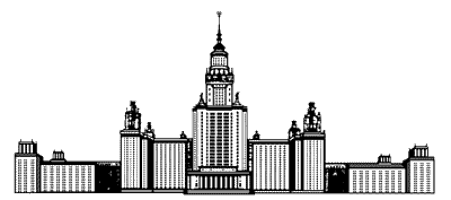
\includegraphics[width = 0.5\linewidth] {msu_logo}
    \end{center}
    \begin{center} 
        Москва, 2024 
    \end{center}
	\thispagestyle{empty} %отсутсвие нумерации на странице

    \newpage
    \tableofcontents %оглавление

    \thispagestyle{empty} %отсутсвие нумерации на странице

    \newpage
    \pagenumbering{arabic} % тип последующей нумерации 
    \section{Постановка задачи}
    Требуется реализовать два метода сортировки одномерного массива: \\
    1. Сортировка методом простого выбора \\
    2. Быстрая сортировка основанная на рекурсивной реализации\\ 
    Сравнить асимптотическую сложность данных алгоритмов и на основе полученных результатов предоставить таблицу сравнений.

    \newpage
    \section{Результаты экспериментов}
    В результате проведенных экспериментов была подтверждена асимптотическая
    оценка алгоритмов: \\
    1. Selection sort $O(n\cdot(n-1)/2)$ \\
    2. Quick sort $O(n\cdot\log_2n)$\\

    TABLE



    \begin{figure}[H]
        \centering
    \begin{tikzpicture}[scale=0.8]
        \begin{axis}[
            name=plot1,
            title={Linear search},
            xlabel={Array length},
            ylabel={t, ms},
            legend pos=north west,
            ymajorgrids=true,
            xmajorgrids=true,
            grid style=dashed,
        ]
        
        \addplot[
            color=red,
            label=l1,
            ]
            coordinates {
                (100,1)(105,2)
            };
            \addlegendentry{worst}
        \addplot[
            color=blue,
            label=l1,
            ]
            coordinates {
                (100,1)(105,0)	
			};
            \addlegendentry{average} % добавление в легенду

        \end{axis}
        \begin{axis}[
            name=plot2,
            at=(plot1.outer south east),  % расположение anchor относительно первого
            anchor=outer south west, % расположение anchor относительно второго 
            title={Binary search},
            xlabel={Array length},
            ylabel={t, ms},
            legend pos=south east,
            ymajorgrids=true, % сетка 
            xmajorgrids=true, % сетка
            grid style=dashed,
        ]
        \addplot[
            color=red,
            label=l1,
            smooth,
            ]
            coordinates {
                (100,51)(105,51)
            };
            \addlegendentry{worst}
        \addplot[
            color=blue,
            label=l1,
            smooth,
            ]
            coordinates {
                (100,48)(105,48)
            };
            \addlegendentry{average}

        \end{axis}
    \end{tikzpicture}
    \end{figure}

    \vspace{1cm}
    \textbf{Вывод:} \\
    \text{ЧТООООООООООо} 


    \newpage
    \section{Структура программы и спецификация функций}
    Для более оптимизированной работы программы использовалтись функции, которые работали как с массивом данных, так и с численными перменными.
    \textbf{Список функций:}\\
    \begin{enumerate}
        \item change() -- функция меняет местами два элемента массивов, которые ей подаются.
        \item selection\_sort() -- функция сортирует массив методом выбора и подсчитывает количество изменений и сравнений, которые были при этом сделаны.
        \item fast_sort() -- функция сортирует массив методом быстрой сортировки рекурсией и подсчитывает количество изменений и сравнений, которые были при этом сделаны.
        \item sort_q() -- сортирует массив по возрастанию, используя selection sort.
        \item sort_rev() -- сортирует массив в обратнмо порядке, используя selection sort.
        \item filling() -- заполняет массив случайным числами, используя условие, которое было выбрано.
    \end{enumerate}

    \end{align*}
    \newpage
    \section{Отладка программы, тестирование программы}

    \newpage
    \section{Анализ допущенных ошибок}

    \newpage
    \section{Литература}

    \begin{thebibliography}{10}
        \bibitem{}
        Трифонов Н. П., Пильщиков В. Н. Задания практикума на ЭВМ (1 курс). Методическая разработка(составители). — М.: ВМК МГУ, 2001.
        \bibitem{}
        Кормен Т., Лейзерсон Ч., Ривест Р., Штайн К. Алгоритмы: построение и анализ. Второе издание.
        — М.: «Вильямс», 2005.
        \bibitem{}
        Головинов Г.  Основы программирования на TeX. Том 1. Начало. — М.: МФТИ, 2024.
        \bibitem{}
        Кнут Д. Искусство программирования для ЭВМ. Том 3. — М.: Мир, 1978.
        \bibitem{}
        Лорин Г. Сортировка и системы сортировки. — М.: Наука, 1983.
    \end{thebibliography}

    


\end{document}

